\documentclass[fontset=ubuntu]{ctexbeamer}

\usepackage{%
  bookmark,
  booktabs,
  datetime2
}

\usepackage{fontawesome5}
\usepackage{hologo}
\usepackage{qrcode}

\usepackage{%
  listings,
  ragged2e
}

\usepackage{graphicx}
\graphicspath{{./figures/}{./showcase/}}

\usepackage{amsmath}
\usepackage{unicode-math}
\usepackage{libertinus}

\setlength\abovecaptionskip{-5pt}
\setlength\belowcaptionskip{-5pt}

\usepackage{tipa}
\usepackage{xpinyin}

\usepackage{dirtree}

\usepackage{xeCJKfntef}

\usepackage{gbt7714}
\bibliographystyle{gbt7714-numerical}

\usetheme{Xiaoshan}
\usefonttheme{serif,professionalfonts}

\setbeamerfont{title}{size=\LARGE, series=\bfseries}
\setbeamerfont{subtitle}{size=\normalsize}

\setbeamertemplate{title}{%
\raggedleft%
\linespread{1.0}%
\inserttitle%
\hspace*{0.75cm}\par%
\vspace*{0.25cm}
}

\setbeamertemplate{subtitle}{%
\raggedleft%
\insertsubtitle%
\hspace*{0.75cm}\par%
\vspace*{0.25cm}
}

\setbeamertemplate{frame numbering}{\zhnumber[style=Ancient]{\insertframenumber}}
\setbeamertemplate{note page}[plain]

% \setbeameroption{show only notes}
% \setbeameroption{show notes on second screen}

\setbeamercolor{block title}{fg=松花绿}
\setbeamersize{description width=2em}

\setCJKmainfont{Noto Serif CJK SC}[
  UprightFont    = * SemiBold,
  BoldFont       = * Black,
  ItalicFont     = * SemiBold,
  BoldItalicFont = * Black,
  CharacterWidth = Full]
\setCJKsansfont{Noto Sans CJK SC}
\setCJKmonofont{Noto Sans CJK SC}

\newcommand{\link}[1]{\href{#1}{\tiny \faLink}}
\newcommand{\pkg}[1]{\texttt{#1}}

\newcommand{\dd}{\symrm{d}}
\newcommand{\V}[1]{\symbf{#1}}

\newcommand{\XeTeX}{\hologo{XeTeX}}
\newcommand{\pdfTeX}{\hologo{pdfTeX}}
\newcommand{\LuaTeX}{\hologo{LuaTeX}}
\newcommand{\XeLaTeX}{\hologo{Xe}\kern-.13em\LaTeX{}}
\newcommand{\pdfLaTeX}{pdf\LaTeX{}}
\newcommand{\LuaLaTeX}{Lua\LaTeX{}}
\newcommand{\BibTeX}{\hologo{BibTeX}}
\newcommand{\hithesis}{\textsc{hi}\-\textsc{Thesis}}

% 颜色
\colorlet{keyword}{松花绿}
\colorlet{comment}{漆黑!50}
\colorlet{texcs}{酡红}
\colorlet{emph1}{靛蓝}
\colorlet{emph2}{琥珀}
\colorlet{inline}{玄色}

% 代码清单
\lstdefinestyle{style@latex}{
  language     = [latex]TeX,
  alsoletter   = {*},
  keywordstyle = \bfseries\color{keyword},
  commentstyle = \color{comment},
  texcsstyle   = *\color{texcs},
  emphstyle    = [1]\color{emph1},
  emphstyle    = [2]\color{emph2}
}
\lstdefinestyle{style@inline}{
  basicstyle   = \ttfamily\color{inline},
  keepspaces   = true
}
\lstnewenvironment{texcode}[1][]{\lstset{
  style        = style@latex,
  basicstyle   = \footnotesize\ttfamily,
  gobble       = 2,
  backgroundcolor=\color{white},
  morekeywords = {\documentclass,\usepackage,\begin,\end},#1
  }
}{}
\lstMakeShortInline[style=style@inline]|

\title{\LaTeX{} 论文排版技术入门}
\subtitle{What You Think Is What You Get}

\author{石佳乐}
\institute{哈尔滨工业大学(威海)}
% \institute{\normalsize
% 1. \LaTeX{} 发展历史与特点\\
% 2. 快速上手不废话(通过示例讲解常用功能)\\
% 3. 论文模板的使用(以哈工大学位论文为例)\\
% 4. 穿插讲解扩展性知识以及使用技巧}
% \date{\zhtoday}
\date{2022 年 6 月 2 日}

\begin{document}

\maketitle

\section{引言}

\subsection{\TeX{} 与 \LaTeX}

\begin{frame}[fragile]{\TeX{} 与 \LaTeX}
  \begin{columns}[T]
    \column{.8\textwidth}
    \begin{itemize}
      \item \TeX{}
            \begin{itemize}
              \item 生成精美图书的排版系统
              \item 最初由 Donald Knuth(高德纳)于 1978 年开发
              \item 每 7 年发布新版,最新版本为 \TeX{} 3.141592653(2021 年 1 月)\link{https://tex.stackexchange.com/questions/581118/whats-new-in-tex-version-3-141592653}
              \item 漂亮、美观、稳定、通用
              \item 尤其擅长数学公式排版
            \end{itemize}
      \item \LaTeX{}
            \begin{itemize}
              \item Leslie Lamport 开发的一种 \TeX{} 格式
              \item 原版 \TeX{} 过于晦涩难懂,\CJKsout{不适合正常人类}
              \item 在 \TeX{} 的基础上提供更多命令,降低使用门槛
              \item 极其丰富的宏包,提供扩展功能
              \item 广泛用于学术界,有各种论文模板
                    % \item 大学学位论文模板,如 \hithesis
            \end{itemize}
    \end{itemize}
    \column{.2\textwidth}
    \vspace*{5mm}
    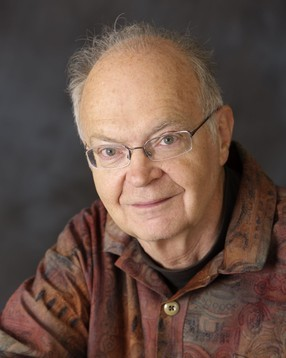
\includegraphics[width=\textwidth]{Knuth.jpg}

    \vspace*{5mm}
    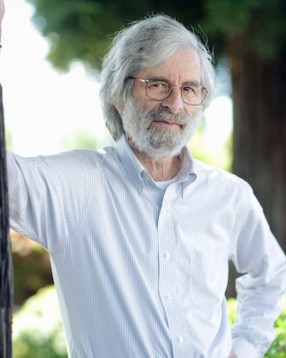
\includegraphics[width=\textwidth]{Lamport.jpg}

  \end{columns}
\end{frame}

\begin{frame}[fragile]{没什么用的知识}
  \begin{itemize}
    \item 关于名字
          \begin{itemize}
            \item \TeX{} 这个名字来源于希腊语词根 τεχ--
            \item \LaTeX{} 则比较简单粗暴:La 就是 Lamport 的意思
          \end{itemize}
    \item 关于读音
          \begin{itemize}
            \item Knuth 坚持要求将 \TeX{} 读作 \textipa{/tEx/},类似“泰赫”
            \item 不过 Lamport 认为 \LaTeX{} 的读音无所谓
          \end{itemize}
    \item 关于拼写
          \begin{itemize}
            \item \TeX{} 一般都会拼成这样错落有致的样子,主要是为了:
                  \begin{itemize}
                    \item 通过奇奇怪怪的排版效果,说明这是一个排版系统的名字
                    \item 与其他名字区分开,比如当年还有一个叫 TEX 的系统
                  \end{itemize}
            \item 如果环境不支持这种排版,则应该拼写为 TeX
            \item 后来 \TeX{} 的衍生产品往往都有类似的做法
                  \begin{itemize}
                    \item \LaTeX{}、\BibTeX{}、\XeTeX{}、\CTeX{}……
                  \end{itemize}
          \end{itemize}
  \end{itemize}
\end{frame}

% \begin{frame}{和 Word 对比}
%   注:术业有专攻,评价需客观
%   \begin{table}[h]
%     \centering
%     % \rowcolors[]{1}{primaryL}{primaryL!40}
%     \begin{tabular}{c|c}
%       Microsoft\textsuperscript{\textregistered}  Word & \LaTeX{}        \\
%       \hline
%       字处理工具                                            & 专业排版软件        \\
%       容易上手,简单直观                                        & 容易上手          \\
%       所见即所得                                            & 所见即所想,所想即所得   \\
%       高级功能不易掌握                                         & 进阶难,但一般用不到    \\
%       处理长文档需要丰富经验                                      & 和短文档处理基本无异    \\
%       花费大量时间调格式                                        & 无需担心格式,专心作者内容 \\
%       公式排版差强人意                                         & 尤其擅长公式排版      \\
%       二进制格式,兼容性差                                       & 文本文件,易读、稳定    \\
%       付费商业许可                                           & 自由免费使用        \\
%     \end{tabular}
%   \end{table}
% \end{frame}

\subsection{\LaTeX{} 排版展示}

\begin{frame}[fragile]{\LaTeX{} 用起来究竟什么样?}
  \vspace{1em}
  \begin{columns}
    \begin{column}{0.55\textwidth}
      \begin{texcode}[gobble=8,basicstyle=\tiny\ttfamily, moretexcs={\maketitle},emph={[1]equation,itemize,document}, emph={[2]article,amsmath,graphicx}]
        \documentclass{article}
        \usepackage{amsmath,graphicx}
        \title{Normal distribution}
        \author{Wikipedia, the free encyclopedia}

        \begin{document}
          \maketitle
          \section{Introduction}
          % 省略一些内容……
          The probability density of the normal
          distribution is
          \begin{equation}
            f(x|\mu, \sigma)
            = \frac{1}{\sqrt{2\pi\sigma^2}}
            e^{-\frac{(x-\mu)^2}{2\sigma^2}}
          \end{equation}
          where
          \begin{itemize}
            \item $\mu$ is the mean of the distribution
            \item $\sigma$ is the standard deviation
          \end{itemize}
        \end{document}
      \end{texcode}
    \end{column}

    \begin{column}{0.45\textwidth}
      \begin{figure}
        \centering
        \vspace{-0.8cm}
        \includegraphics[width=\textwidth, trim={2cm 2cm 2cm 2cm}, clip]%
        {examples/normal-dist/normal-dist.pdf}
      \end{figure}
    \end{column}
  \end{columns}
  % \nonumberfootnote{来源:Wikipedia \link{https://en.wikipedia.org/wiki/Normal_distribution}}
\end{frame}

% \begin{frame}{基本原则}
%   \begin{itemize}
%     \item 排版 vs 文字处理
%           \begin{itemize}
%             \item 《别把 \LaTeX{} 当 Word 用》
%           \end{itemize}
%     \item 遵循业(xué)界(xiào)规范
%           \begin{itemize}
%             \item 《管教务处 or 研究生院 or 物理系叫爸爸》
%           \end{itemize}
%           % \item 追求良好的阅读体验\zhparen{readability}
%     \item 内容与格式分离
%     \item \alert{内容永远比格式重要!}
%           \begin{itemize}
%             \item \emph{Typography exists to honor content.} ---R. Bringhurst
%           \end{itemize}
%   \end{itemize}
% \end{frame}

\begin{frame}{\LaTeX{} 排版展示:文本}
  \vspace{1em}
  \begin{columns}
    \begin{column}{.45\textwidth}
      \begin{figure}
        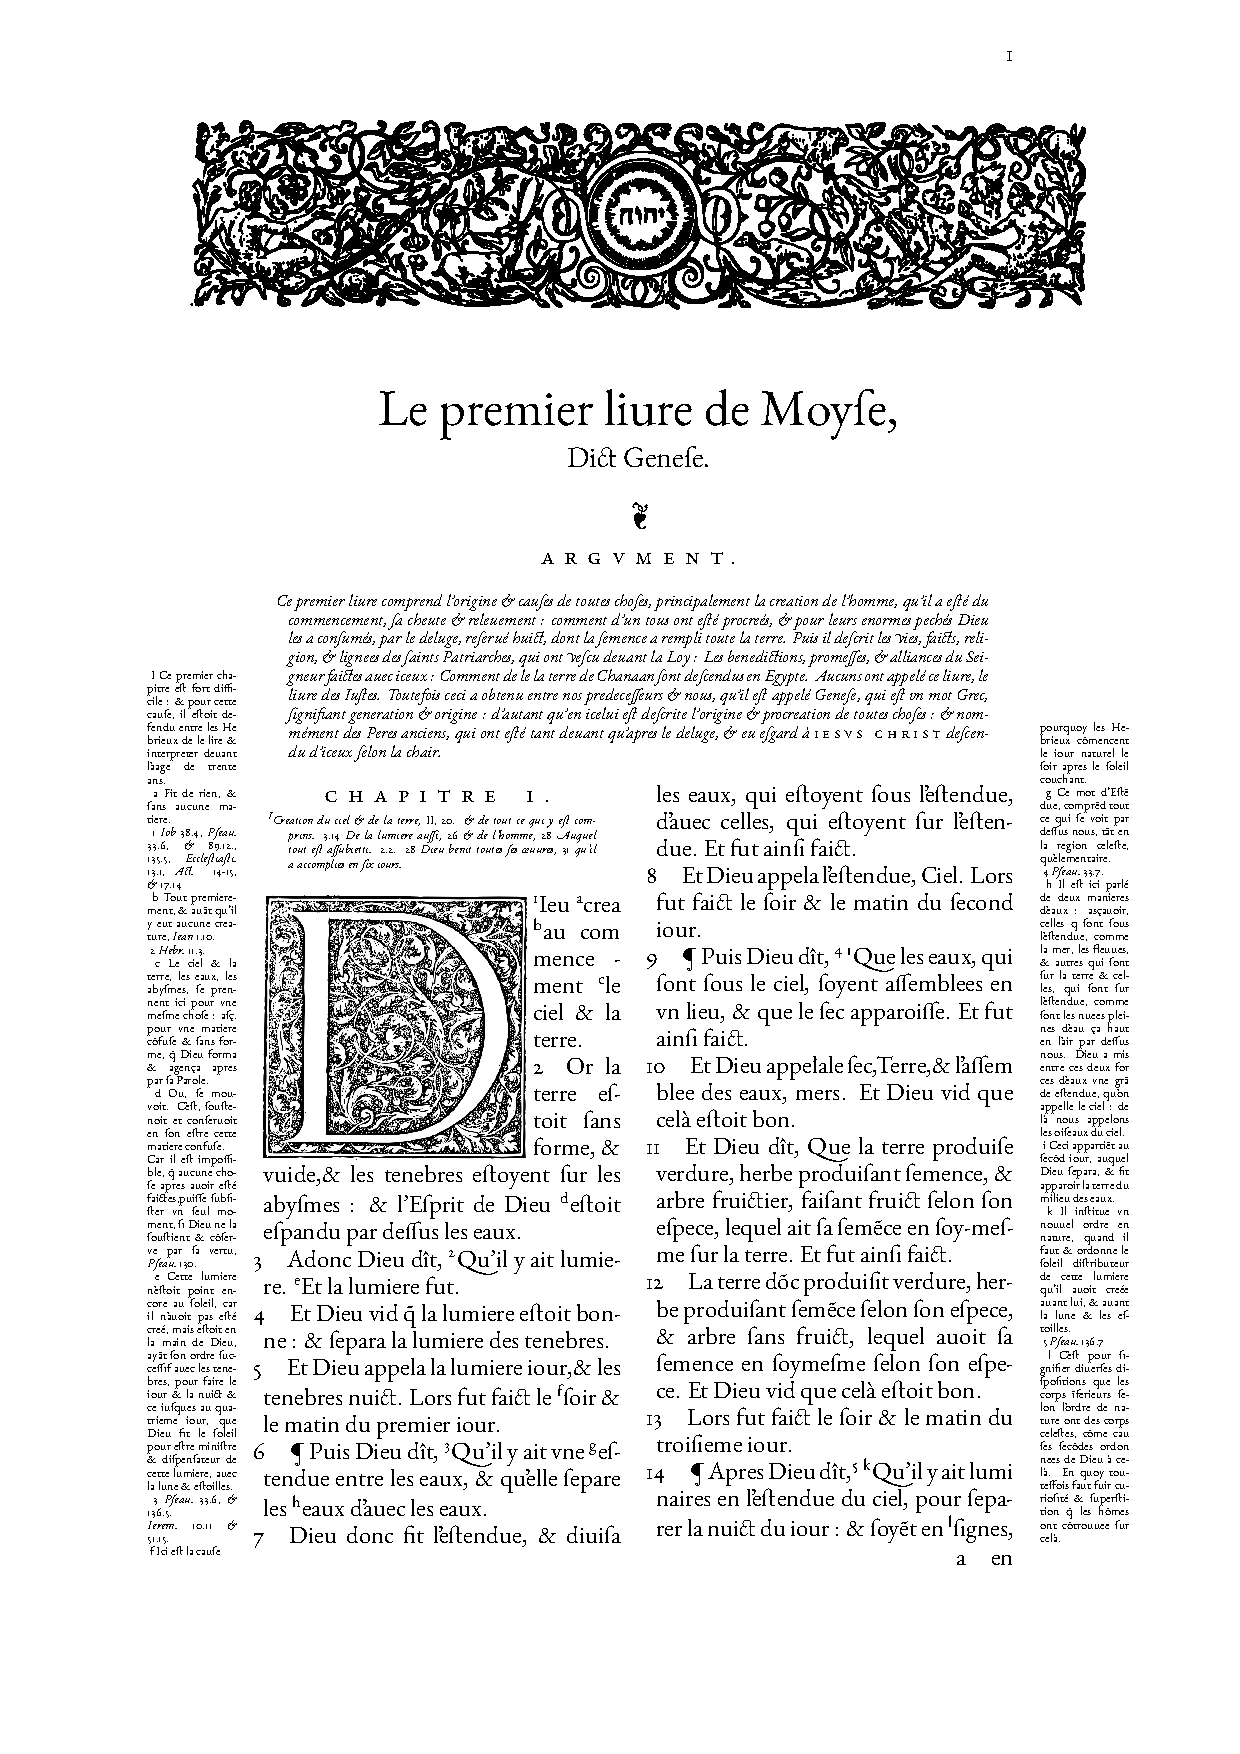
\includegraphics[width=\textwidth,page=1]{geneve_1564.pdf}
      \end{figure}
    \end{column}
    \begin{column}{.45\textwidth}
      \begin{figure}
        \includegraphics[width=\textwidth,page=2]{geneve_1564.pdf}
      \end{figure}
    \end{column}
  \end{columns}
\end{frame}

\begin{frame}{\LaTeX{} 排版展示:公式}
  \begin{align*}
    \oiint_{\partial\Omega} \V{E} \cdot \dd \V{S}
     & = \frac{1}{\epsilon_0} \iiint_\Omega \rho \, \dd V      \\
    \oiint_{\partial\Omega} \V{B} \cdot \dd \V{S}
     & = 0                                                     \\
    \oint_{\partial\Sigma} \V{E} \cdot \dd \V{l}
     & = -\frac{\dd}{\dd t} \iint_\Sigma \V{B} \cdot \dd \V{S} \\
    \oint_{\partial\Sigma} \V{B} \cdot \dd \V{l}
     & = \mu_0 \left( \iint_\Sigma \V{J} \cdot \V{S}
    + \epsilon_0 \frac{\dd}{\dd t} \iint_\Sigma \V{E} \cdot \dd \V{S} \right)
  \end{align*}
\end{frame}

\begin{frame}{\LaTeX{} 排版展示:图形}
  \begin{figure}
    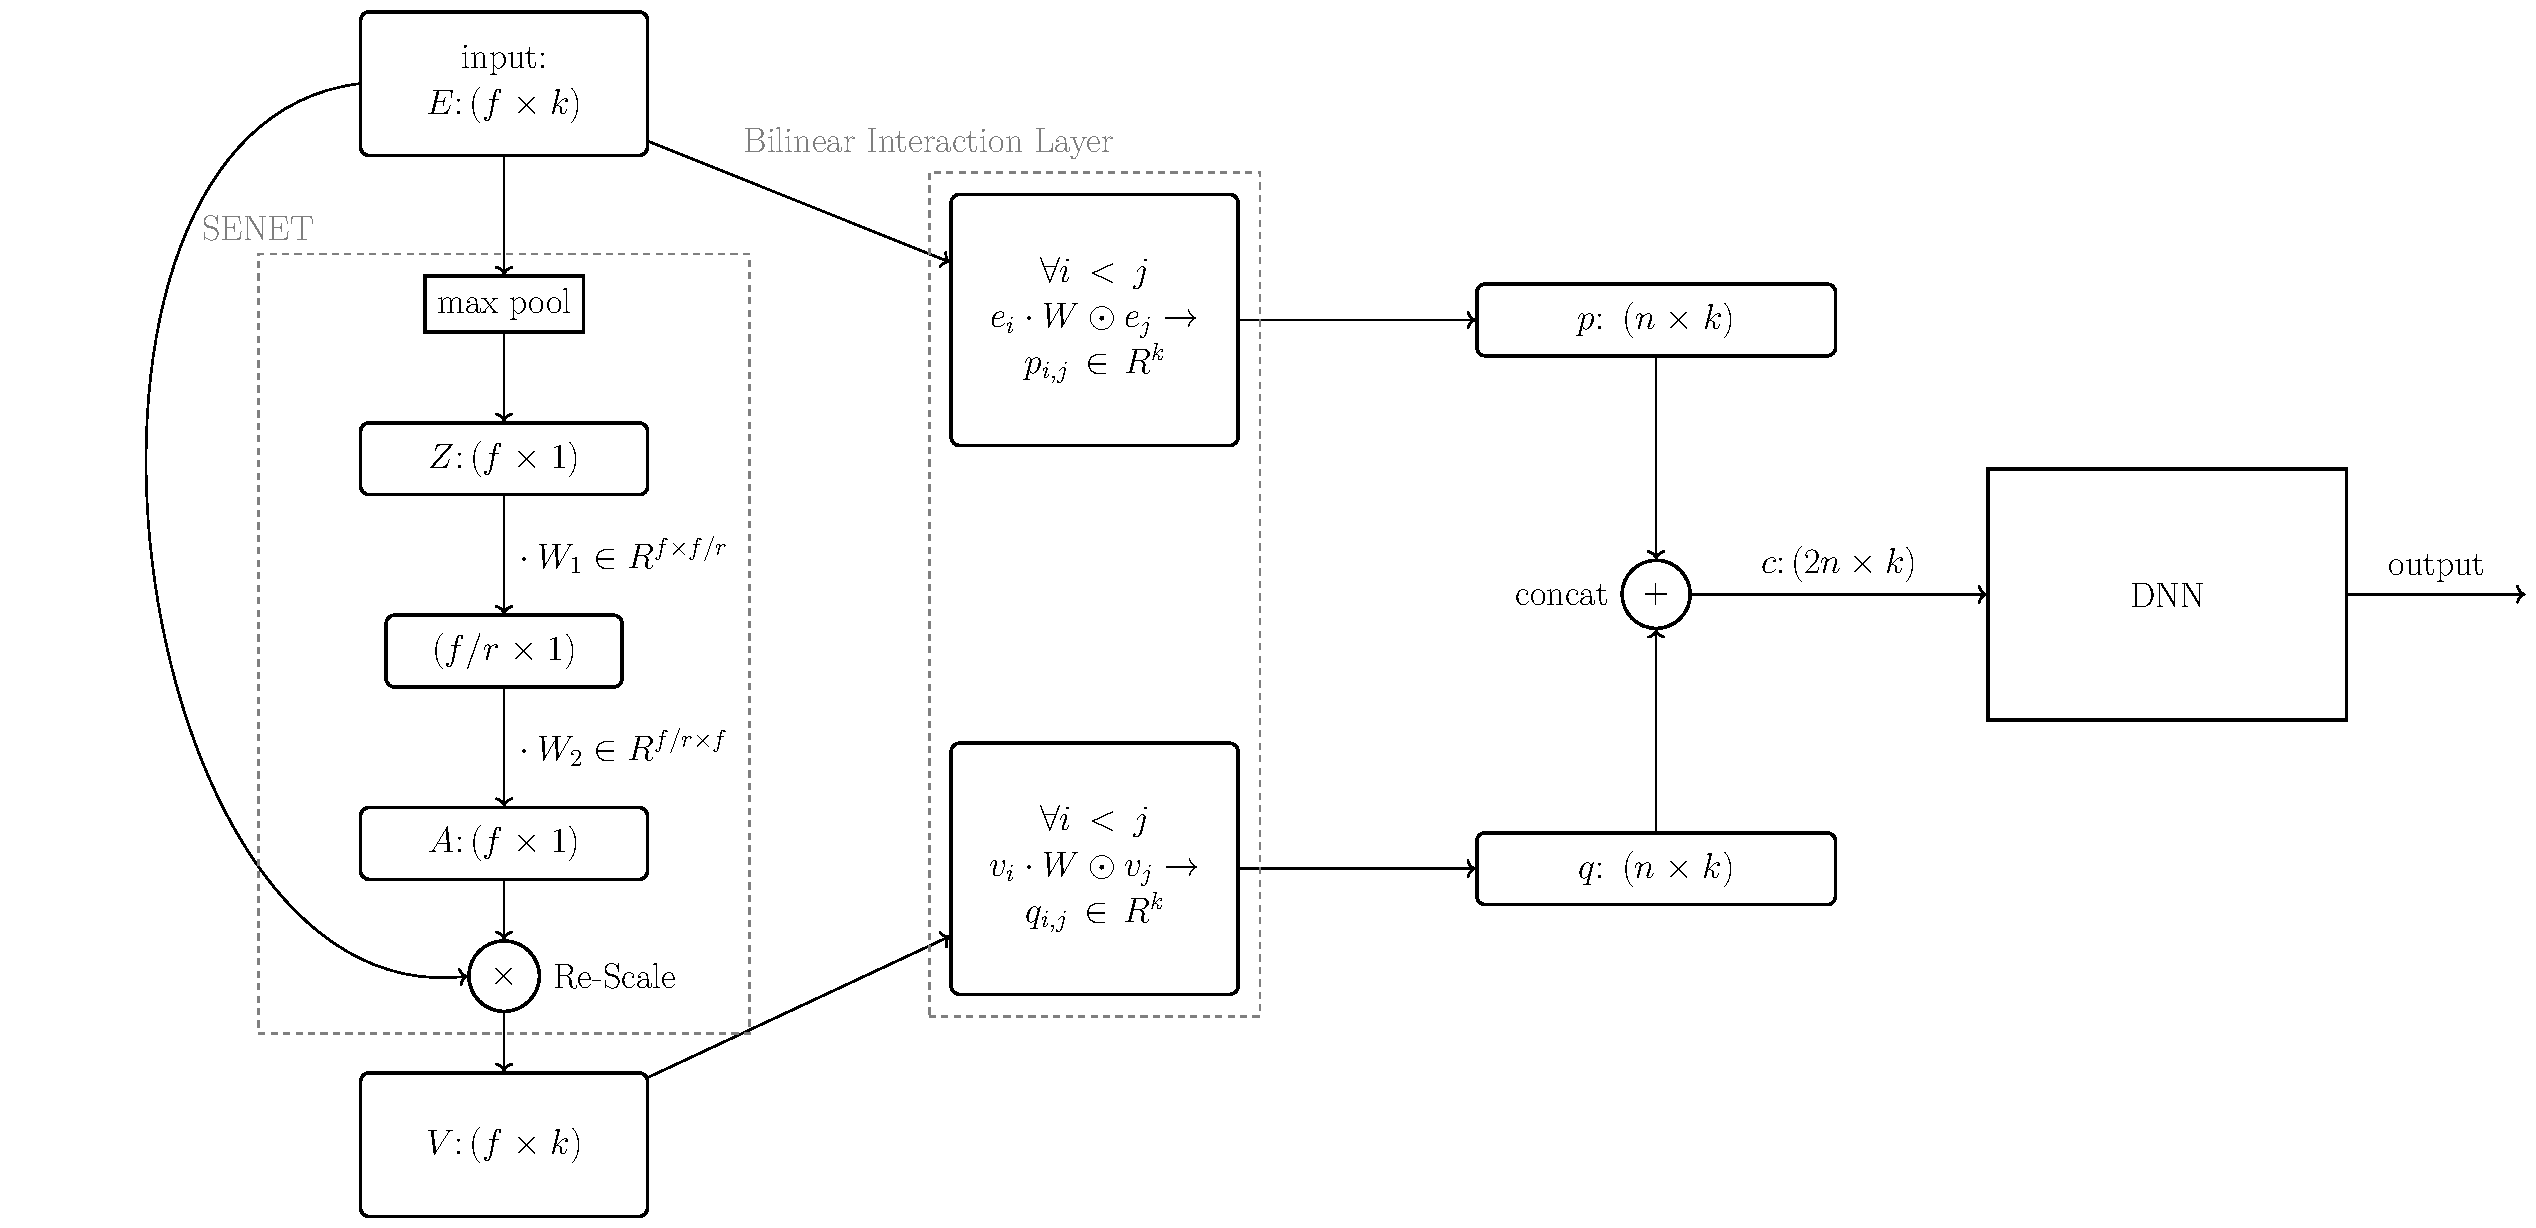
\includegraphics[width=\textwidth]{flowchart.pdf}
  \end{figure}
\end{frame}

\begin{frame}{\LaTeX{} 排版展示:幻灯片}
  \begin{columns}
    \begin{column}{.5\textwidth}
      \begin{figure}
        
\includegraphics[width=\textwidth]{slides_xiaoshan.pdf}
      \end{figure}
    \end{column}
    \begin{column}{.5\textwidth}
      \begin{figure}
        
\includegraphics[width=\textwidth]{slides_hit.pdf}
      \end{figure}
    \end{column}
  \end{columns}
\end{frame}

\begin{frame}{\LaTeX{} 排版展示:简历}
  \vspace{1em}
  \begin{columns}
    \begin{column}{.45\textwidth}
      \begin{figure}
        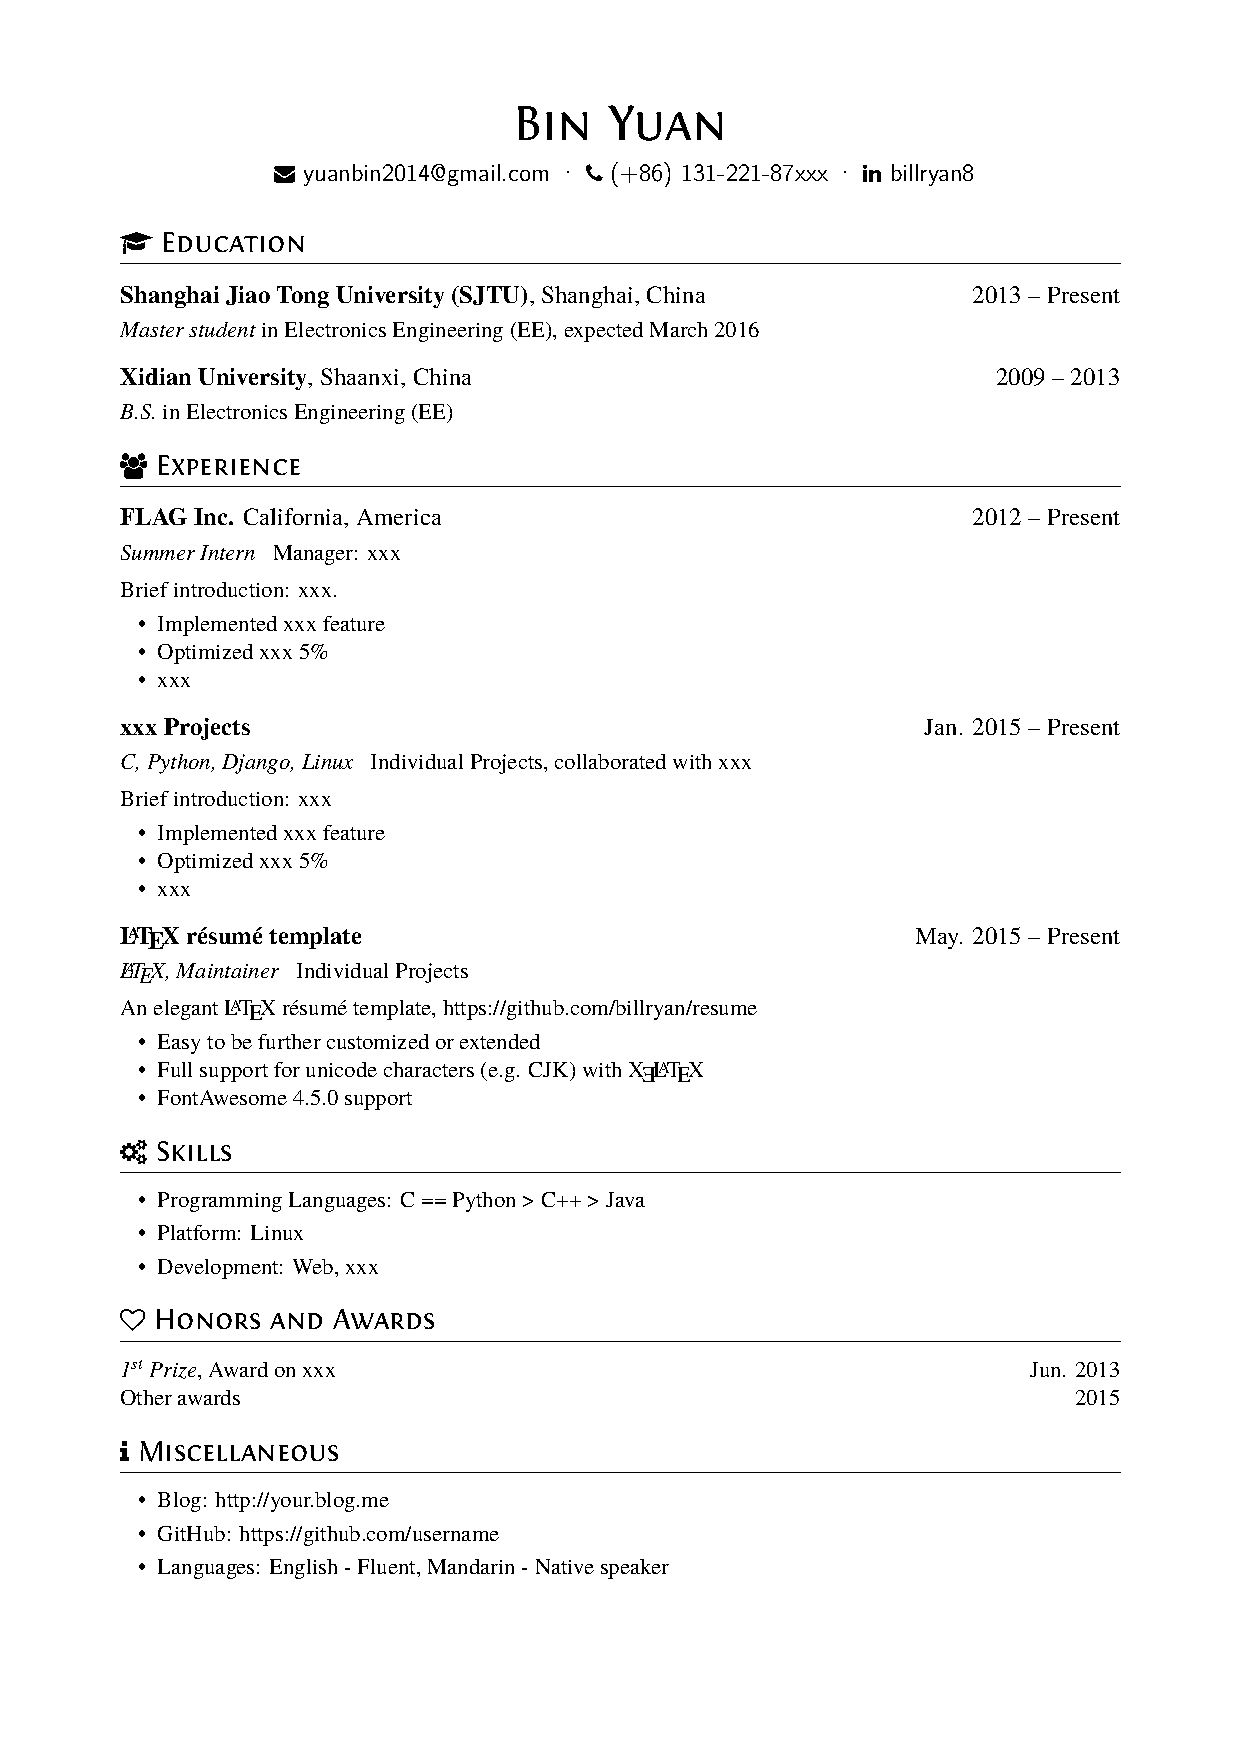
\includegraphics[width=\textwidth]{resume.pdf}
      \end{figure}
    \end{column}
    \begin{column}{.45\textwidth}
      \begin{figure}
        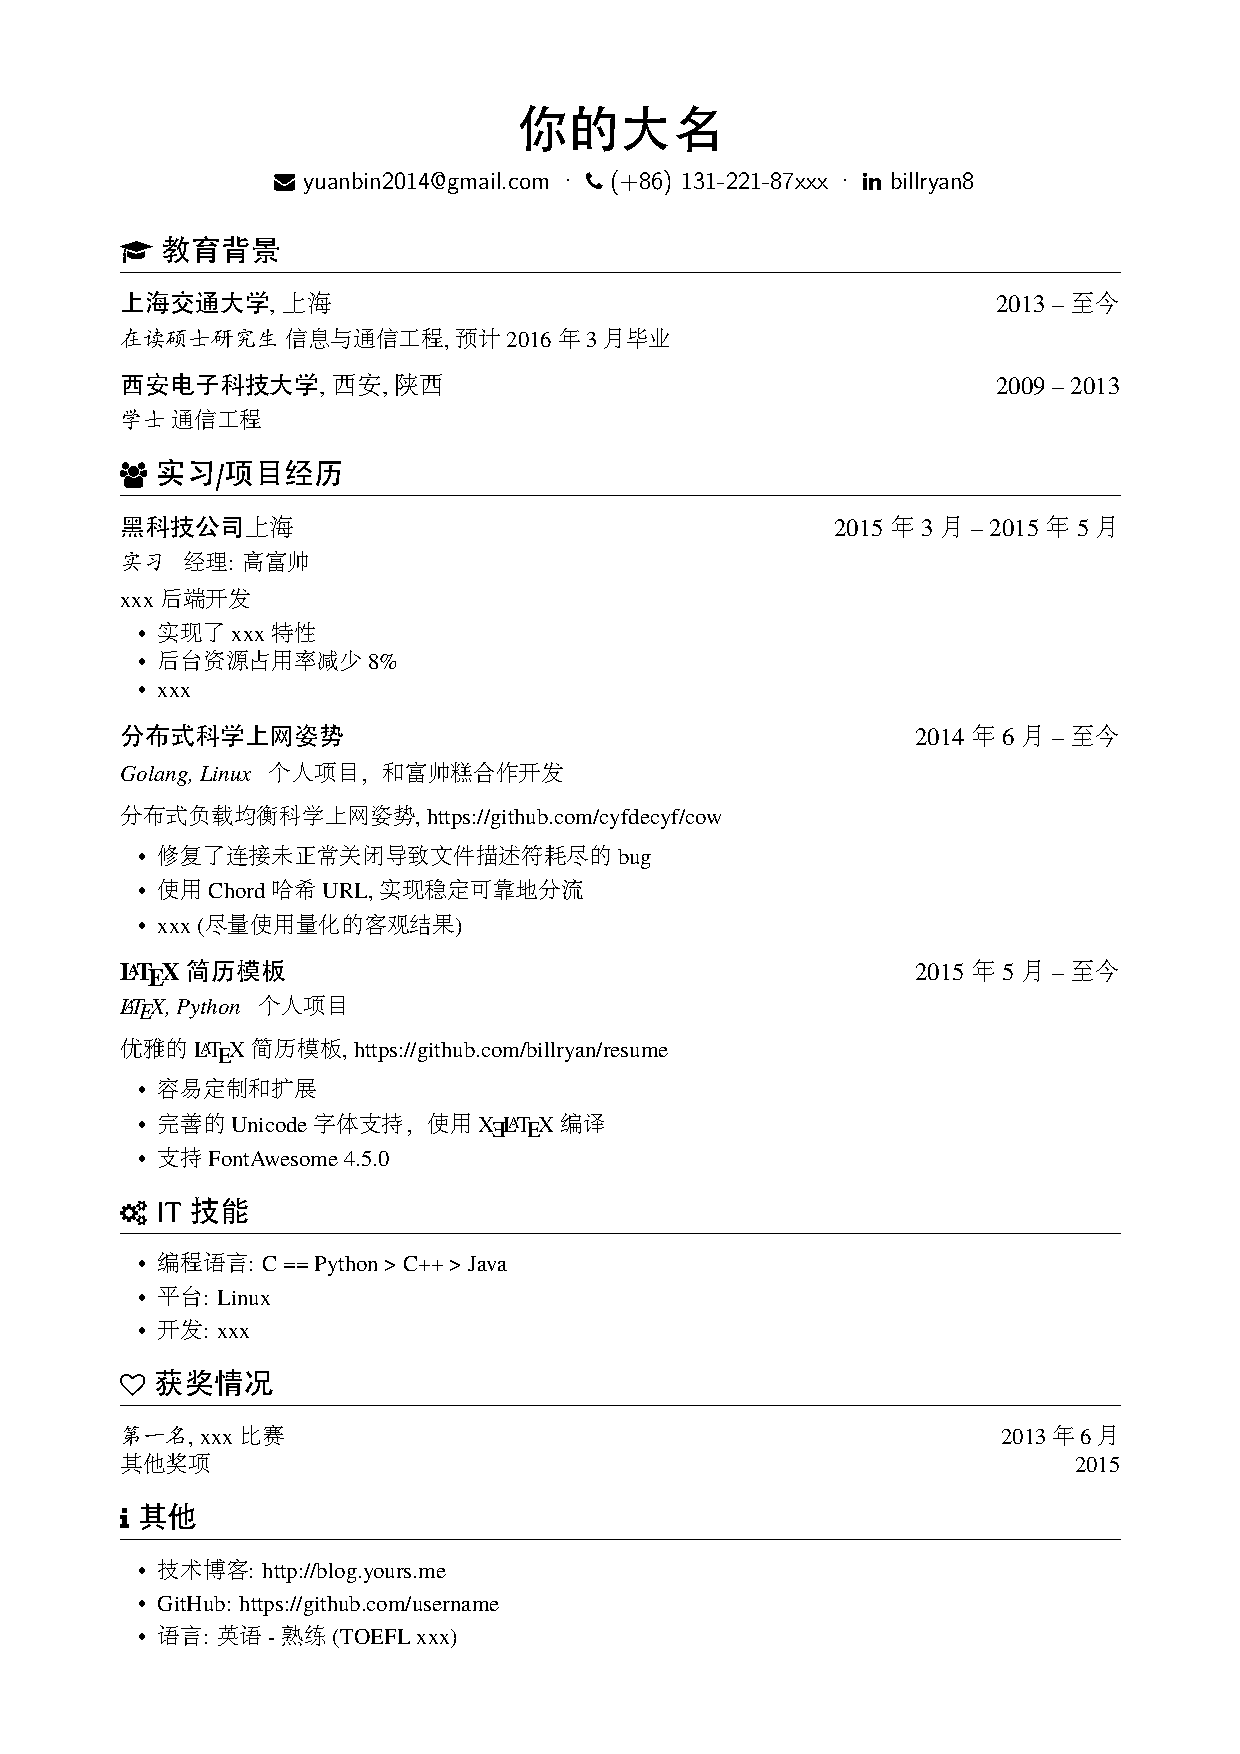
\includegraphics[width=\textwidth]{resume-zh_CN.pdf}
      \end{figure}
    \end{column}
  \end{columns}
\end{frame}

% \begin{frame}{\LaTeX{} 排版示例:公式}
%   \begin{align*}
%     \oiint_{\partial\Omega} \V{E} \cdot \dd \V{S}
%      & = \frac{1}{\epsilon_0} \iiint_\Omega \rho \, \dd V
%      & \quad                                              &
%     \oint_{\partial\Sigma} \V{E} \cdot \dd \V{l}
%     = -\frac{\dd}{\dd t} \iint_\Sigma \V{B} \cdot \dd \V{S} \\
%     \oiint_{\partial\Omega} \V{B} \cdot \dd \V{S}
%      & = 0
%      & \quad                                              &
%     \oint_{\partial\Sigma} \V{B} \cdot \dd \V{l}
%     = \mu_0 \iint_\Sigma \V{J} \cdot \V{S}
%     + \mu_0 \epsilon_0 \frac{\dd}{\dd t} \iint_\Sigma \V{E} \cdot \dd \V{S}
%   \end{align*}
% \end{frame}

\section{快速上手}

\subsection{凡例}

\begin{frame}{凡例}
  术语的第一次出现通常会使用\textbf{粗体}。
  网页链接用\ {\tiny \faLink} 符号表示。

  \begin{block}{扩展}
    这里是扩展性的内容,一般不会影响使用,但能了解是最好的。
  \end{block}

  \begin{alertblock}{注意}
    这里是需要注意的内容,与排版中可能出现的问题相关。
  \end{alertblock}

  \begin{exampleblock}{示例}
    这里是示例,通常以代码加效果的形式出现。
  \end{exampleblock}
\end{frame}

\subsection{安装指南 \& 不安装指南}

\begin{frame}[fragile]{安装指南}
  \begin{enumerate}
    \item 下载:推荐下载\TeX{} Live 的 ISO 镜像离线安装
          \begin{itemize}
            \item 清华大学开源软件镜像站 \link{https://mirrors.tuna.tsinghua.edu.cn/CTAN/systems/texlive/Images/texlive.iso}
            \item 中国科学技术大学开源软件镜像站 \link{https://iso.mirrors.ustc.edu.cn/CTAN/systems/texlive/Images/texlive.iso}
            \item 或者其他镜像站
          \end{itemize}
    \item 安装:建议新手安装完整版
          \begin{itemize}
            \item 以管理员权限运行 |install-tl-windows.bat|
            \item 一路点击“下一步”
            \item 保持耐心
          \end{itemize}
    \item 编辑器:再安装一个合适的编辑器
          \begin{itemize}
            \item 专用型:TeXworks、TeXstudio、TeXShop、Kile……
            \item 通用型:Visual Studio Code、Vim、Emacs……
          \end{itemize}
  \end{enumerate}
  更详细的安装教程:\link{https://mirrors.tuna.tsinghua.edu.cn/CTAN/info/install-latex-guide-zh-cn/install-latex-guide-zh-cn.pdf}

  \note{
    \begin{itemize}
      \item 有很多人推荐其他的 \LaTeX{} 发行版,TeX Live 的确有种种缺点:
            \begin{itemize}
              \item 默认占用空间太大,会安装一堆你可能永远用不到的内容
              \item 对宏包的管理不够方便
              \item Windows 下 TeX Live 版本升级不方便
              \item ……
            \end{itemize}
      \item 但我为新手只推荐 TeX Live 完整版,主要是因为:
            \begin{itemize}
              \item 包含所有常用的宏包、文档、字体等,避免后续的麻烦
              \item 用户基数大,这意味着当你遇到问题时,可以更快地找到解决方案
            \end{itemize}
    \end{itemize}
  }
\end{frame}

\begin{frame}{不安装指南}
  \begin{itemize}
    \item 懒得安装?没关系!
    \item 已经 2202 年了,云端服务可能更好用
    \item 免去安装、配置、升级等一系列烦恼,可以多人协作
    \item 国际平台:Overleaf \link{https://cn.overleaf.com/}
          \begin{itemize}
            \item 老牌服务,成熟稳定,模板丰富
            \item 缺少部分中文字体(例如 Windows 自带的中易系列字体)
          \end{itemize}
    \item 国内平台:TeXPage \link{https://www.texpage.com}
          \begin{itemize}
            \item 默认支持更多的中文字体
            \item 自带免费的数学符号选择器
            \item 不够成熟,收录的模板也较少
          \end{itemize}
  \end{itemize}

  \note{
    \begin{itemize}
      \item 推荐先使用在线环境体验 \LaTeX{}
    \end{itemize}
  }
\end{frame}

\subsection{基本使用方法}

\begin{frame}[fragile]{简单的英文文档}
  \begin{exampleblock}{示例}
    \begin{texcode}[gobble=6,basicstyle=\small\ttfamily,emph={[1]document}, emph={[2]article}]
      % 用 pdfLaTeX、XeLaTeX 或 LuaLaTeX 编译
      \documentclass{article}

      \begin{document}
        Hello World!
      \end{document}
    \end{texcode}
  \end{exampleblock}
\end{frame}

\begin{frame}[fragile]{\LaTeX{} 文档的组成部分}
  \begin{enumerate}
    \item 导言区
          \begin{itemize}
            \item 以 |\documentclass{文档类名}| 开头
            \item \textbf{文档类}定义了这个文档的基本格式
            \item 在导言区,你还可以:
                  \begin{itemize}
                    \item 加载宏包,这样就能在正文中使用更多功能
                    \item 调整格式,因为文档类不一定满足你的需求
                  \end{itemize}
            \item \alert{导言区绝不能出现正文,否则会报错}
          \end{itemize}
    \item 正文区
          \begin{itemize}
            \item 以 |\begin{document}| 开头
                    \item 以 |\end{document}| 结尾
            \item 所有正文内容都要放在这里
            \item 原则上来说,正文区只负责内容,不要在此调整格式
          \end{itemize}
  \end{enumerate}
\end{frame}

\begin{frame}[fragile]{简单的中文文档}
  \begin{exampleblock}{示例}
    \begin{texcode}[gobble=6,basicstyle=\small\ttfamily,emph={[1]document}, emph={[2]ctexart}]
      % 用 XeLaTeX 或 LuaLaTeX 编译
      \documentclass{ctexart}

      \begin{document}
        你好,世界!
      \end{document}
    \end{texcode}
  \end{exampleblock}

  \begin{alertblock}{注意}
    \begin{itemize}
      \item 确保文件编码是 UTF-8
      \item 务必使用 |ctexart| 等中文文档类
    \end{itemize}
  \end{alertblock}

  \note{
    \begin{itemize}
      \item 编写中文文档与英文文档的区别:
            \begin{itemize}
              \item 必须使用 \CTeX{} 宏集提供的中文文档类:ctexart、ctexrep、ctexbook 和 ctexbeamer
              \item 加载 xeCJK 等宏包也可以达到效果,但不推荐
              \item 千万不要用一个叫做 \CTeX{} 套装的东西,那玩意儿太古老了
              \item 必须用 \XeLaTeX 等引擎编译
            \end{itemize}
    \end{itemize}
  }
\end{frame}

\begin{frame}[fragile]{基本语法}
  \begin{description}
    \item[注释] 以 |%| 开头,其后所有内容都会被忽略
    \item[命令] 以 |\| 开头,区分大小写,可以提供内容或格式
      \begin{itemize}
        \item |\foo|:有些命令可以不带参数直接使用
        \item |\foo{arg}|:必需参数放在大括号 |{...}| 内
        \item |\foo[bar]{arg}|:可选参数放在中括号 |[...]| 内
      \end{itemize}
    \item[环境] 为一整块内容提供特定的格式
      \begin{texcode}[gobble=8, emph={[1]env}]
        \begin{env}
          ...
        \end{env}
      \end{texcode}
  \end{description}
  \vspace{-1em}
  \begin{alertblock}{注意}
    \begin{itemize}
      \item 有些符号在 \LaTeX{} 中有特殊的作用,因此不能直接输入\\
            需要\textbf{转义}:如用 |\%| 表示 |%|、|\textbackslash| 表示 |\| 等
      \item 连续多个空格 = 单个空格、单个换行符 = 单个空格
            % \item 命令和环境都可以自行定义或修改,但要小心行事
    \end{itemize}
  \end{alertblock}

  \note{
    \begin{itemize}
      \item 一个命令可能既有必需参数,也有可选参数
      \item 有多个参数时,参数的位置是固定的,不能随便放
            % \item 例如,如果一个命令格式是 |\foo[bar]{arg}|,就绝对不能写成 |\foo{arg}[bar]|
    \end{itemize}
  }
\end{frame}

\begin{frame}[fragile]
  \frametitle{谋篇布局}
  \begin{itemize}
    \item 文档部件
          \begin{itemize}
            \item 标题:|\title|、|\author|、|\date| $\rightarrow$ |\maketitle|
            \item 目录:|\tableofcontents|
            \item 章节:|\chapter|、|\section|、|\subsection| 等
            \item 文献:|\bibliography|
          \end{itemize}
    \item 文档划分
          \begin{itemize}
            \item 凤头猪肚豹尾:|\frontmatter|、|\mainmatter|、|\backmatter|
            \item 分文件编译:|\include|、|\input|
          \end{itemize}
  \end{itemize}
\end{frame}

\begin{frame}[fragile]
  \frametitle{文本标记}
  \begin{itemize}
    \item 字体相关
          \begin{itemize}
            \item 字号:|\tiny|、|\small|、|\large|、|\Large| 等
            \item 加粗:|{\bfseries ...}| 或 |\textbf{...}|
            \item 倾斜:|{\itshape ...}| 或 |\textit{...}|
          \end{itemize}
    \item 段落相关
          \begin{itemize}
            \item 换行:|\\|
            \item 换段:空行或 |\par|
            \item 换页:|\newpage|
                  % \item 缩进:|\indent|
            \item 居中:|\centering| 或 |center| 环境
          \end{itemize}
  \end{itemize}
\end{frame}

\begin{frame}[fragile]{一个更完善的文档}
  \vspace{-1em}
  \begin{exampleblock}{示例}
    \begin{texcode}[gobble=6,basicstyle=\small\ttfamily,emph={[1]document}, emph={[2]ctexart}]
      \documentclass{ctexart}

      \title{这是文章标题}
      \author{这是作者}
      \date{这是日期}

      \begin{document}
        % 在导言区定义标题内容后,在正文区生成标题
        \maketitle
        \section{这是第一节的标题}
        你好,世界!

        这是另一段。
      \end{document}

    \end{texcode}
  \end{exampleblock}
\end{frame}

\begin{frame}[fragile]{命令是如何起作用的?}
  \begin{block}{扩展}
    \begin{itemize}
      \item 计算机编程中的\textbf{宏}
            \begin{itemize}
              \item 可以将一段内容替换为另一段内容,这一过程称为\textbf{宏展开}
            \end{itemize}
      \item \TeX{} 就是一种基于宏的系统
            \begin{itemize}
              \item \TeX{} 排版引擎只能解析有限的命令,它们称为\textbf{原始命令}
              \item 其他命令都是宏,最终会被层层展开以供排版引擎处理
              \item \LaTeX{} 提供了额外的宏,各种宏包、用户也可以自定义宏
            \end{itemize}
    \end{itemize}
  \end{block}
  \vspace{-1em}
  \begin{exampleblock}{示例}
    \begin{itemize}
      \item 为什么 |\TeX| 命令能输出错落有致的排版效果(\TeX)?
      \item 因为它会被展开成下面这一堆代码:\\
            \footnotesize |T\kern -.1667em\lower .5ex\hbox {E}\kern -.125emX|
    \end{itemize}
  \end{exampleblock}

  \note{
    \begin{itemize}
      \item 宏可以大大简化代码的编写
    \end{itemize}
  }
\end{frame}

\begin{frame}[fragile]{引擎与格式}
  \vspace{-1em}
  \begin{block}{扩展}
    \begin{itemize}
      \item \textbf{引擎}:\TeX{} 的实现,是幕后真正干活(排版)的程序
            \begin{itemize}
              \item \pdfTeX{}:直接生成 PDF,支持 micro-typography
              \item \XeTeX{}:支持 Unicode、OpenType 与复杂文字编排(CTL)
              \item \LuaTeX{}:支持 Unicode、OpenType,内联 Lua
              \item (u)p\TeX{}:日本方面推动,生成 |.dvi|,(支持 Unicode)
            \end{itemize}
      \item \textbf{格式}:\TeX{} 的语言扩展(命令封装)
            \begin{itemize}
              \item plain \TeX{}:Knuth 同志专用
              \item \LaTeX{}:排版科技类文章的事实标准
              \item Con\TeX{t}:基于 \LuaTeX{} 实现,优雅、易用(吗?)
            \end{itemize}
      \item \textbf{发行版}:把引擎、格式、宏包、文档等各种东西打包到一起
            \begin{itemize}
              \item TeX Live:官方维护,跨平台,首选
              \item MacTeX:约等于 macOS 下的 TeX Live
              \item MiKTeX:个人维护,特点是宏包可以随装随用
                    % \item \textbf{程序}:引擎 + dump 之后的格式代码
                    %       \begin{itemize}
                    %         \item \alert{英文文章:\pdfLaTeX{}、\XeLaTeX{} 或 \LuaLaTeX{}}
                    %         \item \alert{中文文章:\XeLaTeX{} 或 \LuaLaTeX{}}
                    %       \end{itemize}
            \end{itemize}
    \end{itemize}
  \end{block}
\end{frame}

\subsection{常用元素}

\begin{frame}[fragile]{常用元素:列表}
  \begin{exampleblock}{示例}
    \begin{columns}
      \begin{column}{0.45\textwidth}
        \begin{texcode}[gobble=10, emph={[1]enumerate,itemize}]
          \begin{enumerate}
            \item 自由软件的定义
              \begin{itemize}
                \item 自由度〇
                \item 自由度一
                \item 自由度二
                \item 自由度三
              \end{itemize}
            \item 自由和非自由的边界
            \item 自由软件定义的实践
          \end{enumerate}
        \end{texcode}
      \end{column}

      \begin{column}{0.45\textwidth}
        % \footnotesize
        \begin{enumerate}
          \item 自由软件的定义
                \begin{itemize}
                  \item 自由度〇
                  \item 自由度一
                  \item 自由度二
                  \item 自由度三
                \end{itemize}
          \item 自由和非自由的边界
          \item 自由软件定义的实践
        \end{enumerate}
      \end{column}
    \end{columns}
  \end{exampleblock}

  \note{
    \begin{itemize}
      \item enumerate 环境提供有编号列表,itemize 环境提供无编号列表,description 环境提供描述性列表。
      \item 在列表环境中,每个 \backslash item 命令就是一个条目
      \item 各种列表环境之间可以相互嵌套,示例中就演示了 enumerate 和 itemize 环境的嵌套。
    \end{itemize}
  }
\end{frame}

\begin{frame}[fragile]{常用元素:图片(一)}
  \begin{exampleblock}{示例}
    \begin{columns}
      \begin{column}{0.6\textwidth}
        \begin{texcode}[gobble=10, moretexcs={\graphicspath,\includegraphics},emph={[1]figure}, emph={[2]graphicx}]
          \usepackage{graphicx}

          % 必需参数为文件名,后缀可省略
          
\includegraphics{figures/logo.png}
        \end{texcode}
      \end{column}

      \begin{column}{0.35\textwidth}
        \centering
        
\includegraphics[width=1.0\textwidth]{logo.png}
      \end{column}
    \end{columns}
  \end{exampleblock}

  \begin{alertblock}{注意}
    \begin{itemize}
      \item 这是最简单的插入图片示例,但不能直接用在排版中。
    \end{itemize}
  \end{alertblock}
\end{frame}

\begin{frame}[fragile]{浮动体}
  \begin{itemize}
    \item 上面的用法有什么问题?
          \begin{itemize}
            \item 将图片直接嵌入文本特定位置,可能严重影响排版效果
            \item 没有标题,不符合论文排版要求
            \item 没有编号,无法方便地进行引用
          \end{itemize}
    \item \textbf{浮动体}机制
          \begin{itemize}
            \item 可以自动将图片、表格等大块内容移动到合适的位置
            \item 支持标题和自动编号等功能
            \item \LaTeX{} 的 |figure| 和 |table| 环境都是浮动体
            \item 浮动体环境的可选参数 |[htbp]| 可以进行位置控制
          \end{itemize}
    \item 浮动体的使用技巧
          \begin{itemize}
            \item 不要强求浮动体“乖乖待在插入的位置”
                  \link{https://liam.page/2017/03/11/floats-in-LaTeX-basic}
            \item 避免“下图”“上表”等表述,而要使用“图 1”“表 1”等
            \item 建议写完全文之后统一调整
          \end{itemize}
  \end{itemize}
\end{frame}


\begin{frame}[fragile]{交叉引用}
  \begin{itemize}
    \item \textbf{交叉引用}
          \begin{itemize}
            \item 被引处:使用 |\label| 定义标签
                  \begin{itemize}
                    \item 图表:紧跟在 |\caption| 命令之后
                    \item 章节:紧跟在 |\section| 等章节命令之后
                    \item 公式:任意位置
                  \end{itemize}
            \item 引用处:使用 |\ref|、|\eqref| 等引用标签,自动获取编号
          \end{itemize}
  \end{itemize}
  \vspace{-1em}
  \begin{alertblock}{注意}
    \begin{itemize}
      \item “我这里没有成功显示‘图 1’,而是‘图~?’,这是咋回事?”
            \begin{itemize}
              \item 因为文档引用了自身内容,一次编译无法获取某些信息
              \item 需要多次编译
                    \begin{itemize}
                      \item 对于简单的交叉引用,通常编译两次即可
                      \item 推荐用 \pkg{latexmk} 自动处理,各种在线环境也采用了此工具
                    \end{itemize}
            \end{itemize}
    \end{itemize}
  \end{alertblock}
\end{frame}

\begin{frame}[fragile]{常用元素:图片(二)}
  \begin{exampleblock}{示例}
    \begin{columns}
      \begin{column}{0.6\textwidth}
        \begin{texcode}[gobble=10, moretexcs={\graphicspath,\includegraphics},emph={[1]figure}, emph={[2]graphicx}]
          % 加载图片宏包
          \usepackage{graphicx}
          % 可以统一指定图片路径
          \graphicspath{{./figures/}}

          如图~\ref{fig_logo} 所示。
          \begin{figure}
            \centering
            % 必需参数为文件名,后缀可省略
            % 可选参数可指定尺寸、裁剪等选项
            
\includegraphics[...]{logo.png}
            \caption{\LaTeX{} 图标}
            \label{fig_logo}
          \end{figure}
        \end{texcode}
      \end{column}

      \begin{column}{0.35\textwidth}
        如图~\ref{fig_logo_} 所示。
        \begin{figure}
          \centering
          
\includegraphics[width=1.0\textwidth]{logo.png}
          \caption{\LaTeX{} 图标}
          \label{fig_logo_}  % Avoid duplicate labels warning
        \end{figure}
      \end{column}
    \end{columns}
  \end{exampleblock}

  \note{
    \begin{itemize}
      \item 这一页幻灯片中涉及的点有很多:
            \begin{itemize}
              \item 加载宏包:宏包能提供更多的宏,方便文档编写,一个宏包通常是为一种特定的功能而设计的
              \item 交叉引用
              \item 浮动体
            \end{itemize}
    \end{itemize}
  }
\end{frame}

\begin{frame}[fragile]{常用元素:图片(三)}
  \begin{itemize}
    \item 外部绘图工具
          \begin{itemize}
            \item Mathematica、MATLAB
            \item PowerPoint、Visio、Adobe Illustrator、Inkscape、Figma 等
            \item Python \texttt{Matplotlib}、\texttt{Plots.jl}、R、Plotly 等
            \item draw.io \link{https://app.diagrams.net/}、
                  Mathcha \link{https://www.mathcha.io}、
                  ProcessOn \link{https://www.processon.com} 等网站
          \end{itemize}
    \item \TeX{} 内联
          \begin{itemize}
            \item Asymptote
            \item \alert{\pkg{pgf}/\pkg{TikZ}、\pkg{pgfplots}}
          \end{itemize}
    \item 插图格式
          \begin{itemize}
            \item 矢量图:|.pdf|%(不再推荐 |.eps|)
            \item 位图:|.png| 或 |.jpg|
            \item 不(完全)支持 |.svg| 和 |.bmp|
            \item \alert{尽量用矢量图}
          \end{itemize}
    \item 参考:\link{https://www.zhihu.com/question/21664179}
          \link{https://tex.stackexchange.com/q/158668}
          \link{https://tex.stackexchange.com/q/72930}
  \end{itemize}
\end{frame}

\begin{frame}[fragile]{常用元素:表格(一)}
  \begin{exampleblock}{示例}
    \begin{columns}
      \begin{column}{0.5\textwidth}
        \begin{texcode}[gobble=10,emph={[1]tabular}]
          \begin{tabular}{cc}
            标题 & 标题 \\
            内容 & 内容 \\
            ...
            内容 & 内容 \\
          \end{tabular}
        \end{texcode}
      \end{column}

      \begin{column}{0.4\textwidth}
        \scriptsize
        \begin{tabular}{cc}
          命令                 & 渲染结果             \\
          |\&|               & \&               \\
          |\%|               & \%               \\
          |\$|               & \$               \\
          |\#|               & \#               \\
          |\_|               & \_               \\
          |\{|               & \{               \\
          |\}|               & \}               \\
          |\textasciitilde|  & \textasciitilde  \\
          |\textasciicircum| & \textasciicircum \\
          |\textbackslash|   & \textbackslash   \\
        \end{tabular}
      \end{column}
    \end{columns}
  \end{exampleblock}

  \begin{alertblock}{注意}
    \begin{itemize}
      \item 这是最简单的插入表格示例,但不能直接用在排版中。
    \end{itemize}
  \end{alertblock}
\end{frame}

\begin{frame}[fragile]{常用元素:表格(二)}
  \vspace{-1em}
  \begin{exampleblock}{示例}
    \begin{columns}
      \begin{column}{0.5\textwidth}
        \begin{texcode}[gobble=10,moretexcs={\toprule,\midrule,\bottomrule},emph={[1]table,tabular}, emph={[2]booktabs}]
          % 绘制三线表的宏包
          \usepackage{booktabs}

          如表~\ref{tab_escape} 所示。
          \begin{table}
            \caption{\LaTeX{} 转义字符}
            \label{tab_escape}
            \begin{tabular}{cc}
              \toprule
              标题 & 标题 \\
              \midrule
              内容 & 内容 \\
              \bottomrule
            \end{tabular}
          \end{table}
        \end{texcode}
      \end{column}

      \begin{column}{0.4\textwidth}
        \scriptsize
        \LaTeX{} 常用转义字符如表~\ref{tab_escape_} 所示。
        \scriptsize
        \begin{table}
          \caption{\LaTeX{} 转义字符}
          \label{tab_escape_}
          \begin{tabular}{cc}
            \toprule
            命令                 & 渲染结果             \\
            \midrule
            |\&|               & \&               \\
            |\%|               & \%               \\
            |\$|               & \$               \\
            |\#|               & \#               \\
            |\_|               & \_               \\
            |\{|               & \{               \\
            |\}|               & \}               \\
            |\textasciitilde|  & \textasciitilde  \\
            |\textasciicircum| & \textasciicircum \\
            |\textbackslash|   & \textbackslash   \\
            \bottomrule
          \end{tabular}
        \end{table}
      \end{column}
    \end{columns}
  \end{exampleblock}

  \note{
    \begin{itemize}
      \item booktabs 宏包定义了不同横线的命令,用于绘制三线表
      \item 类似插入图片,注意本示例中对浮动体和交叉引用的使用
    \end{itemize}
  }
\end{frame}

\begin{frame}[fragile]{常用元素:表格(三)}
  \begin{itemize}
    \item |tabular| 环境配合相关宏包可以实现更多表格功能
    \item 手动绘制表格确实比较令人头疼,且较难维护
    \item 可以使用在线工具生成表格代码:Tables Generator \link{https://www.tablesgenerator.com/}
  \end{itemize}
  \begin{block}{扩展}
    \begin{itemize}
      \item 除了基本的 |tabular| 环境外,也有宏包提供其他表格环境
      \item 特别推荐 \pkg{tabularray} 宏包
            \begin{itemize}
              \item 兼容性好
              \item 功能强大,各种需求皆可轻松实现
            \end{itemize}
    \end{itemize}
  \end{block}
\end{frame}

\section{公式}

\subsection{数学模式}

\begin{frame}[fragile]{数学模式}
  \begin{itemize}
    \item 一切公式都要在\textbf{数学模式}下输入
          \begin{itemize}
            \item 提供了公式排版所需的命令和特性
            \item 数学模式的字体设置独立于文本模式
            \item 间距根据符号类型自动调整,空格会被忽略,空行会报错
          \end{itemize}
    \item \textbf{行内公式}
          \begin{itemize}
            \item 公式与文字混排
            \item 用一对美元符号包裹:|$...$|
            \item 示例:理想气体状态方程可以写为 $PV=nRT$, 其中 $P$、$V$ 和 $T$ 分别是压强、体积和绝对温度
          \end{itemize}
    \item \textbf{行间公式}
          \begin{itemize}
            \item 公式单独成行
            \item 无编号:|\[...\]| 或 |equation*| 环境
            \item 带编号:|equation| 环境
          \end{itemize}
  \end{itemize}
\end{frame}

\subsection{公式排版}

\begin{frame}[fragile]{结构}
  \begin{itemize}
    \item 上标:|^{上标}|
    \item 下标:|_{下标}|
    \item 分式:|\frac{分子}{分母}|
    \item 根式:|\sqrt[根指数]{根底数}|
  \end{itemize}

  \begin{exampleblock}{示例}
    \begin{columns}
      \begin{column}{0.7\textwidth}
        \begin{texcode}[gobble=10, emph={[1]enumerate,itemize}]
          % gather 是一个常用的多行公式环境
          \begin{gather*}
            (\sqrt[n]{a})^{n}=a \\
            \log_{a}b=\frac{\log_{c}b}{\log_{c}a}
          \end{gather*}
        \end{texcode}
      \end{column}

      \begin{column}{0.25\textwidth}
        \vspace*{-2em}
        \begin{gather*}
          (\sqrt[n]{a})^{n}=a \\
          \log_{a}b=\frac{\log_{c}b}{\log_{c}a}
        \end{gather*}
      \end{column}
    \end{columns}
  \end{exampleblock}
\end{frame}


\begin{frame}[fragile]{括号(定界符)}
  \begin{itemize}
    \item 基本括号
          \begin{itemize}
            \item |(...)|、|[...]|、|\{...\}|
            \item 绝对值、范数:|...| 或 |\vert...\vert|、|\Vert...\Vert|
            \item 尖括号:|<...>| 或 |\langle...\rangle|
          \end{itemize}
    \item 自动调节大小
          \begin{itemize}
            \item |\left(...\right)| 等
            \item 自动匹配内部公式的尺寸
          \end{itemize}
    \item 手动调节大小
          \begin{itemize}
            \item 只有 4 + 1 档:|\big|、|\Big|、|\bigg|、|\Bigg|
            \item 声明左中右:|\bigl|、|\bigm|、|\bigr| 等
            \item 示例:$\Biggl( \biggl( \Bigl( \bigl( () \bigr) \Bigr) \biggr) \Biggr)$
          \end{itemize}
  \end{itemize}

  \note{
    \begin{itemize}
      \item 尽管手动调节时只有几个尺寸可选,但自动调节时大部分定界符都可以无限延伸,实现原理是用多个“零件”拼接起来
    \end{itemize}
  }
\end{frame}

\begin{frame}[fragile]{数学符号}
  \begin{itemize}
    \item 寻找符号
          \begin{itemize}
            \item 最常用的额外字体包:\pkg{amssymb}
            \item 常用符号表:各种入门教程和编辑器通常都会给出
            \item 更多符号表:\textit{The Comprehensive \LaTeX{} Symbol List}
                  \link{https://ctan.org/pkg/comprehensive}
            \item 手写识别(有趣但不全):Detexify \link{http://detexify.kirelabs.org}
          \end{itemize}
    \item 数学字体
          \begin{itemize}
            \item Times New Roman 字体:\pkg{newtxmath} 宏包
                  % \item \alert{不要用 \pkg{times} 和 \pkg{mathptmx} 宏包}
                  % \item 加粗:使用 \pkg{bm} 宏包的 |\bm| 命令(|\mathbf| 只有直立的字母)
          \end{itemize}
  \end{itemize}
  \vspace{-1em}
  \begin{block}{扩展}
    \begin{itemize}
      \item 新方案:\pkg{unicode-math}
            \link{https://stone-zeng.github.io/2020-05-02-use-opentype-fonts-iii}
            \begin{itemize}
              \item 符号、字体、样式精调的一揽子解决方案
              \item 彻底修改底层,不可与传统方案混用
            \end{itemize}
    \end{itemize}
  \end{block}
\end{frame}

% \begin{frame}[fragile]{结构}
%   \begin{itemize}
%     \item 上下标
%           \begin{itemize}
%             \item |^| 和 |_|:|f^ab| 和 |f^{ab}|,|e^x^2|、|{e^x}^2| 和 |e^{x^2}|
%           \end{itemize}
%     \item 分式
%           \begin{itemize}
%             \item |\frac{<分子>}{<分母>}|
%           \end{itemize}
%     \item 根式
%           \begin{itemize}
%             \item |\sqrt[<次数>]{<内容>}|
%             \item 复杂情况改用分数指数:|{...}^{1/n}|
%           \end{itemize}
%     \item 矩阵与行列式
%           \begin{itemize}
%             \item |matrix|、|pmatrix|、|vmatrix| 等环境
%             \item 语法类似表格:|&| 分列,|\\| 换行
%             \item 推荐 \pkg{physics} 宏包
%           \end{itemize}
%   \end{itemize}
% \end{frame}

\begin{frame}[fragile]{公式排版技巧}
  \begin{itemize}
    \item 建议始终调用 \pkg{amsmath} 宏包
    \item \lstinline[style=style@inline]|\(no)limits| 命令可以调整积分、求和、极限等元素(|\int|、|\sum|、|\lim|)的显示方式
          \begin{itemize}
            \item $\sum\limits_{i=0}^n {x_i}$ 对比 $\sum\nolimits_{i=0}^n {x_i}$
          \end{itemize}
    \item 小分式、行内分式不好看:改用 |a/b|、或改用行间公式
    \item 手动调节括号大小往往比自动调节更好看
    \item \alert{不建议用 MathType 生成 \LaTeX{} 公式}
    \item \alert{不要用 \texttt{\$\$...\$\$}}
          % \item \alert{不推荐 \texttt{\textbackslash dfrac}}
  \end{itemize}
\end{frame}

\section{论文排版}

\subsection{引用与参考文献}

\begin{frame}[fragile]{引用与参考文献(〇)}
  \begin{description}
    \item[引用] 在正文中出现,用于指出附加信息,十分简短
    \item[参考文献] 在文末出现,用于提供附加信息,按一定顺序罗列
  \end{description}
\end{frame}

\begin{frame}[fragile]{引用与参考文献(一)}
  \begin{enumerate}
    \item 将参考文献条目存储在 |.bib| 文件中
          \begin{itemize}
            \item 每个条目包含文献类型、基本信息以及一个用于引用的键值
            \item 看起来很复杂,但其实不用手动输入
                  \begin{itemize}
                    \item 各种文献管理工具都可以批量导出 |.bib| 格式的条目
                    \item 谷歌学术等文献搜索网站也可以直接复制
                    \item \CJKsout{知网居然连这功能都没有}
                  \end{itemize}
          \end{itemize}
    \item 在文章中添加引用和参考文献
          \begin{itemize}
            \item 导言区
                  \begin{itemize}
                    \item 指定样式:|\bibliographystyle{样式名}|
                    \item 国家标准 GB/T 7714--2015
                          \link{https://github.com/Haixing-Hu/GBT7714-2005-BibTeX-Style/files/153951/GBT.7714-2015.pdf}:
                          \pkg{gbt7714} 宏包
                          %         \item 更多文献、引用样式:\pkg{natbib} 宏包
                  \end{itemize}
            \item 正文区
                  \begin{itemize}
                    \item 标记引用:|\cite{键值}|
                    \item 插入参考文献:|\bibliography{.bib 文件名}|
                  \end{itemize}
          \end{itemize}
  \end{enumerate}
\end{frame}

\begin{frame}[fragile]{引用与参考文献(二)}
  \begin{exampleblock}{示例:\texttt{.bib} 文件}
    \begin{texcode}[gobble=6]
      @incollection{1844_marx_manuscripts,
        author    = {马克思},
        title     = {1844年经济学哲学手稿},
        booktitle = {马克思恩格斯全集},
        publisher = {人民出版社},
        year      = 2002,
        editor    = {马克思 and 恩格斯},
        volume    = 3,
        pages     = {266-280},
        edition   = 2,
        address   = {北京},
        language  = {zh}
      }
    \end{texcode}
  \end{exampleblock}
\end{frame}

\begin{frame}[fragile]{引用与参考文献(三)}
  \begin{exampleblock}{示例:在文章中添加引用和参考文献}
    \begin{texcode}[gobble=6]
      马克思分析了异化劳动的四个方面。\cite{1844_marx_manuscripts}

      \bibliography{reference.bib}
    \end{texcode}
    \vspace{1em}
    \hspace{2em}马克思分析了异化劳动的四个方面。\cite{1844_marx_manuscripts}
    \begin{center}
      \zihao{3} \textsf{参考文献}
    \end{center}
    \renewcommand{\bibsection}{}
    \bibliography{reference.bib}
  \end{exampleblock}
\end{frame}

\begin{frame}[fragile]{引用与参考文献(四)}
  \begin{alertblock}{注意}
    \begin{itemize}
      \item “我都编译了好几次了,怎么还不能正常显示呢?”
            \begin{itemize}
              \item 处理 |.bib| 并非 \TeX{} 引擎本身功能,而要靠 \BibTeX 程序
              \item 通常要先用 \TeX{} 和 \BibTeX 分别编译一遍,再继续用 \TeX{} 编译
              \item 例如:\XeLaTeX $\rightarrow$ \BibTeX $\rightarrow$ \XeLaTeX $\rightarrow$ \XeLaTeX
              \item 再次推荐 \pkg{latexmk}
            \end{itemize}
    \end{itemize}
  \end{alertblock}
  \vspace{-1em}
  \begin{block}{扩展}
    \begin{itemize}
      \item \BibTeX 后端是处理参考文献的传统方法,但功能受限
      \item 更新的方法:\pkg{biber} 后端 + \pkg{biblatex} 宏包
      \item 不过很多模板目前依然采用 \BibTeX,请根据情况选择
    \end{itemize}
  \end{block}
\end{frame}

\subsection{论文模板}

\begin{frame}[fragile]{模板}
  \begin{itemize}
    \item 是什么?
          \begin{itemize}
            \item 设计好的格式框架,可以让用户专注于内容
                  % \item Word 中的样式:「学好 \LaTeX{} 可以更科学地使用 Word」
            \item 以文档类的形式提供,扩展名为 |.cls|
          \end{itemize}
    \item 有哪些?
          \begin{itemize}
            \item 期刊会议:\pkg{revtex}、\pkg{elsarticle}、\pkg{IEEEtran}……
            \item 学位论文:\pkg{thuthesis}、\pkg{ustcthesis}、\hithesis……
          \end{itemize}
    \item 怎么用?
          \begin{itemize}
            \item |\documentclass[模板参数]{模板名}|
            \item 每个模板都可能有独特的用法
                  \begin{itemize}
                    \item \alert{读文档、读文档、读文档}
                    \item \alert{看示例、看示例、看示例}
                  \end{itemize}
          \end{itemize}
    \item 去哪里找?
          \begin{itemize}
            \item 期刊或会议官网
            \item CTAN \link{https://ctan.org} 或 GitHub \link{https://github.com}
            \item 有些模板集成在 TeX 发行版中,但注意确认是否为最新版
          \end{itemize}
  \end{itemize}
\end{frame}

\begin{frame}[fragile]{\hithesis:简介}
  \begin{itemize}
    \item 民间维护的哈工大学位论文 \LaTeX{} 模板
    \item 包括一校三区本科、硕士、博士开题、中期和毕业论文
    \item 生成 PDF 版论文,支持知网查重
    \item 链接:\url{https://github.com/hithesis/hithesis}
    \item 另外,\TeX{} Live 发行版自带本模板,但可能版本滞后
    % \item 未来项目可能迁移至:
    %       \begin{itemize}
    %         \item \url{https://github.com/hithesis/hithesis}
    %       \end{itemize}
  \end{itemize}
\end{frame}

\begin{frame}[fragile]{\hithesis:下载}
  \begin{figure}
    \centering
    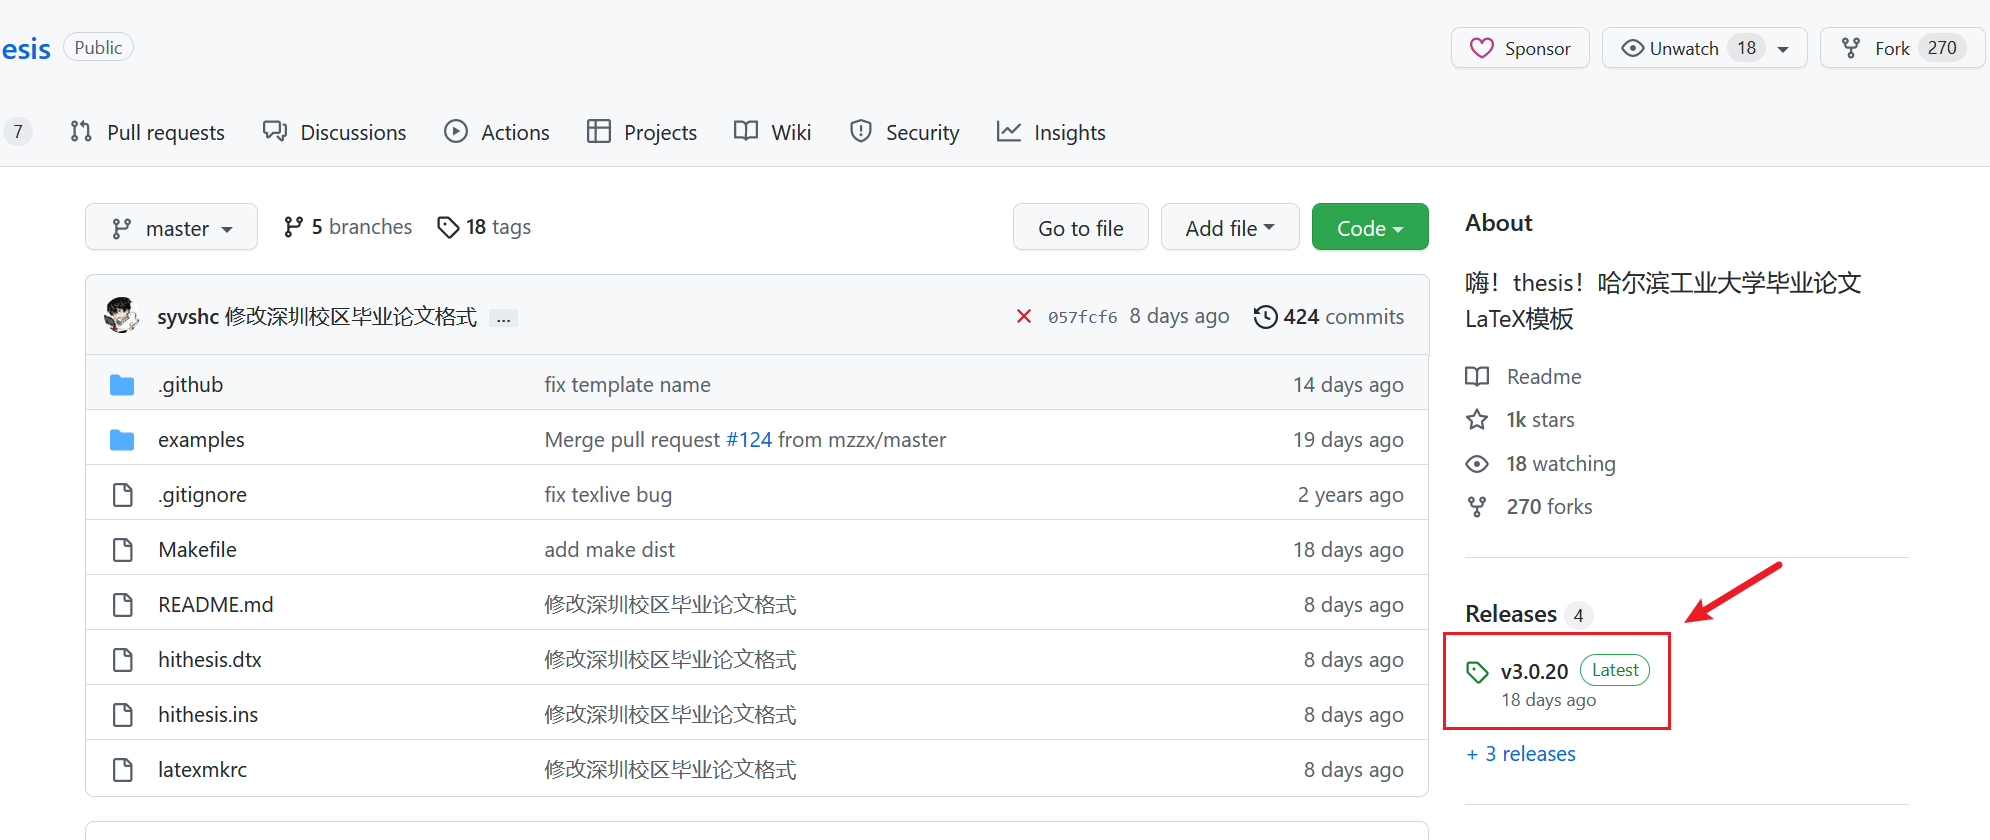
\includegraphics[width=0.8\textwidth]{hithesis_dowload_1.png}
  \end{figure}
  \begin{figure}
    \centering
    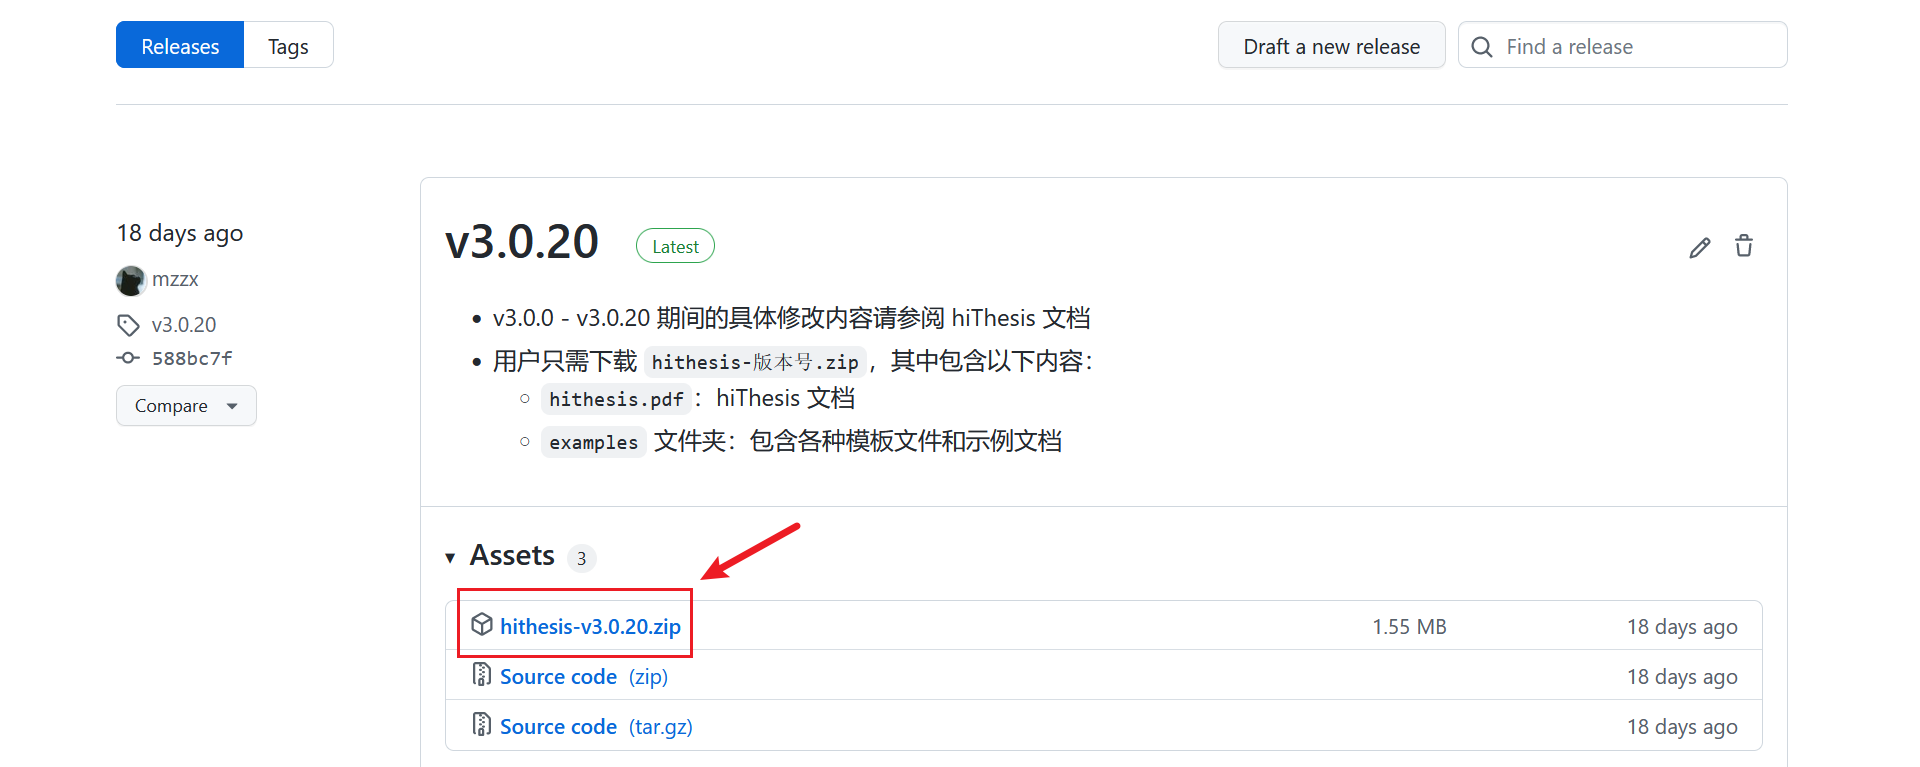
\includegraphics[width=0.8\textwidth]{hithesis_dowload_2.png}
  \end{figure}
\end{frame}

\begin{frame}[fragile]{\hithesis:主目录结构}
  % \dirtree{%
  %   .1 hithesis/.
  %   .2 examples/.
  %   .3 hitart/.
  %   .3 hitbook/.
  %   .2 hithesis.pdf.
  % }
  \hithesis 的主目录结构如下:
  \begin{table}[htbp]
    \begin{tabular}{ll}
      \toprule
      文件名/目录名                           & 描述            \\
      \midrule
      \pkg{example/}                    & 模板示例文件夹       \\
      \pkg{├─ hitart/}                  & 开题和中期报告文件夹    \\
      \pkg{│\phantom{─ }├─ reports/}    & 开题和中期报告文件夹    \\
      \pkg{│\phantom{─ }└─ reportplus/} & 深圳校区博士中期报告文件夹 \\
      \pkg{└─ hitbook/}                 & 毕业论文文件夹       \\
      \pkg{\phantom{├─ }├─ chinese/}    & 中文毕业论文文件夹     \\
      \pkg{\phantom{├─ }└─ english/}    & 英文毕业论文文件夹     \\
      \pkg{hithesis.pdf}                & 用户手册          \\
      \bottomrule
    \end{tabular}
  \end{table}
\end{frame}

% \begin{frame}[fragile]{\hithesis:一个示例的目录结构}
%   \hithesis 示例(以中文毕业论文为例)的目录结构如下:
%   \begin{table}[htbp]
%     \begin{tabular}{ll}
%       \toprule
%       文件名/目录名                           & 描述            \\
%       \midrule
%       \pkg{example/}                    & 模板示例文件夹       \\
%       ├─ \pkg{hitart/}                  & 开题和中期报告文件夹    \\
%       │\phantom{─ }├─ \pkg{reports/}    & 开题和中期报告文件夹    \\
%       │\phantom{─ }└─ \pkg{reportplus/} & 深圳校区博士中期报告文件夹 \\
%       └─ \pkg{hitbook/}                 & 毕业论文文件夹       \\
%       \phantom{│─ }├─ \pkg{chinese/}    & 中文毕业论文文件夹     \\
%       \phantom{│─ }└─ \pkg{english/}    & 英文毕业论文文件夹     \\
%       \pkg{hithesis.pdf}                & 用户手册          \\
%       \bottomrule
%     \end{tabular}
%   \end{table}
% \end{frame}

% \begin{frame}[fragile]{\hithesis:参数}
%   \begin{itemize}
%     \item 常用参数
%           \begin{itemize}
%             \item type\\
%                   doctor/master/bachelor/postdoc\\
%                   (必选)学位:本科/硕士/博士/博士后
%             \item campus\\
%                   shenzhen/weihai/harbin\\
%                   校区:深圳/威海/本部
%             \item fontset\\
%                   windows/mac/ubuntu/fandol/adobe\\
%                   字体:默认会根据系统选择
%           \end{itemize}
%     \item 其他参数请参阅文档
%   \end{itemize}
% \end{frame}

% \begin{frame}[fragile]{\hithesis:开发版}
%   \begin{itemize}
%     \item 常用参数
%           \begin{itemize}
%             \item type\\
%                   doctor/master/bachelor/postdoc\\
%                   (必选)学位:本科/硕士/博士/博士后
%             \item campus\\
%                   shenzhen/weihai/harbin\\
%                   校区:深圳/威海/本部
%             \item fontset\\
%                   windows/mac/ubuntu/fandol/adobe\\
%                   字体:默认会根据系统选择
%           \end{itemize}
%     \item 其他参数请参阅文档
%   \end{itemize}
% \end{frame}

\section{进阶}

\begin{frame}[fragile]{\LaTeX{} 的更多用途}
  \begin{itemize}
    \item 毕竟论文又不是天天写,对吧……
          \pause
    \item 幻灯片
          \begin{itemize}
            \item |beamer| 文档类提供了幻灯片功能(中文用 |ctexbeamer|)
            \item 每个 |frame| 环境生成一个幻灯片页面
            \item |\pause| 命令可以让内容一条一条出现
          \end{itemize}
          \pause
    \item 简历
          \begin{itemize}
            \item 排版出整洁优雅的简历
            \item 网上可以找到各种简历模板,例如:\link{https://github.com/billryan/resume/tree/zh_CN}
          \end{itemize}
          \pause
    \item 笔记
          \begin{itemize}
            \item 特别是笔记中需要很多数学公式时
            \item Markdown 笔记软件通常兼容 \LaTeX{} 的公式格式
            \item 利用 |markdown| 宏包,你甚至可以在 \LaTeX{} 里写 Markdown
          \end{itemize}
  \end{itemize}
\end{frame}

\begin{frame}{\LaTeX{} 系统学习}
  \begin{itemize}
    \item 经典文档
          \begin{itemize}
            \item 仔细阅读《一份不太简短的 \LaTeXe{} 介绍》
                  \link{https://mirrors.tuna.tsinghua.edu.cn/CTAN/info/lshort/chinese/lshort-zh-cn.pdf}
            \item 粗略阅读《\LaTeXe{} 插图指南》
                  \link{https://github.com/WenboSheng/epslatex-cn/blob/master/epslatex-cn.pdf}
          \end{itemize}
    \item 包太雷(黄新刚)\textit{\LaTeX{} Notes}
          \link{https://github.com/huangxg/lnotes/blob/master/lnotes2.pdf}
    \item 刘海洋《\LaTeX{} 入门》
          % \item Stefan Kottwitz \textit{LaTeX Cookbook}
    \item 维基教科书:英文 \link{https://en.wikibooks.org/wiki/LaTeX}、中文 \link{https://zh.wikibooks.org/wiki/LaTeX}
    \item 在线教程:Overleaf 帮助文档
          \link{https://www.overleaf.com/learn}
          % \item 仔细阅读《\hithesis 用户手册》~(20 分钟)
          % \item 从~\hithesis 示例文档入手
  \end{itemize}
\end{frame}

\begin{frame}{一点人生的经验}
  \begin{itemize}
    \item 不要着急安装,先在 Overleaf 或 TeXPage 上熟悉各类操作
    \item 先找个不重要的机会练练手,以免在重要任务中手忙脚乱
    \item 实验室祖传的安装包多半是过时的、\hithesis 八成是旧版的
    \item 写一点儿,编译一次,方便发现和定位错误
    \item 推荐使用 Git 等工具进行版本管理
    \item Windows 系统编译较慢,GNU/Linux 和 macOS 会快很多
    \item \alert{工具是为人服务的,怎么顺手怎么来}(前提是确保用法无误)
    \item \alert{格式是为内容服务的,不要舍本逐末}
  \end{itemize}
\end{frame}

\begin{frame}[fragile]{解决问题之道}
  \begin{enumerate}
    \item 阅读文档
          \begin{itemize}
            \item 使用 |texdoc| 命令即可打开宏包文档
            \item \CJKsout{好吧实际上大多数人都懒得读文档}
          \end{itemize}
    \item 搜索网络
          \begin{itemize}
            \item 优先用英文搜索,有网络条件的请使用谷歌,不行用必应
            \item 用中文百度也可以,但不要过于相信那些社区博客
          \end{itemize}
    \item 提问
          \begin{itemize}
            \item 论坛
                  \begin{itemize}
                    \item \TeX{} - \LaTeX{} Stack Exchange \link{https://tex.stackexchange.com}
                    \item \CTeX{} 临时论坛 \link{https://github.com/CTeX-org/forum}
                    \item \LaTeX{} 工作室 \link{https://www.latexstudio.net}(资源需要甄别,且部分内容需付费)
                  \end{itemize}
            \item 群聊
                  \begin{itemize}
                    \item \hithesis 讨论群:851792460
                  \end{itemize}
            \item 请提供\alert{最小工作示例(MWE,minimal working example)}
          \end{itemize}
  \end{enumerate}
\end{frame}


\begin{frame}{社区参与}
  \begin{itemize}
    \item 参与讨论
          \begin{itemize}
            \item 你的经验也可以解他人之忧
          \end{itemize}
    \item 文档翻译
          \begin{itemize}
            \item \pkg{lshort-zh-cn} \link{https://github.com/CTeX-org/lshort-zh-cn}
            \item \pkg{learnlatex.org/zh} \link{https://github.com/CTeX-org/learnlatex.github.io}
          \end{itemize}
    \item 宏包开发与维护
          \begin{itemize}
            \item 不妨先从修 typo 开始
            \item 欢迎参与维护 \hithesis
          \end{itemize}
    \item \CJKsout{来当主讲人}
  \end{itemize}
\end{frame}

\begin{frame}{关于}
  \vspace*{1cm}
  \footnotesize
  本幻灯片:\url{https://github.com/mzzx/latex-talk}\\
  许可协议:知识共享~署名—相同方式共享 4.0 国际版 \link{https://creativecommons.org/licenses/by-sa/4.0/legalcode.zh-Hans}
  \vspace{0.5cm}
  \begin{center}
    \huge
    \faCreativeCommons\,\faCreativeCommonsBy\,\faCreativeCommonsSa
  \end{center}
  \vspace{1cm}
  \begin{flushleft}
    \tiny
    主题:萧山 \link{https://ctan.org/pkg/pgfornament-han} \\
    正文字体:思源宋体 + Libertinus Serif \\
    等宽字体:思源黑体 + Fira Mono \\
    参考:曾祥东\quad 现代 \LaTeX{} 入门讲座 \link{https://github.com/stone-zeng/latex-talk} \\
    \phantom{参考:}清华大学 TUNA 协会\quad 如何使用 \LaTeX{} 排版论文 \link{https://github.com/tuna/thulib-latex-talk}
  \end{flushleft}
  % \vspace{-0.5cm}
\end{frame}

\begin{frame}
  \begin{center}
    \Huge Happy \LaTeX{ing}!
  \end{center}
\end{frame}


\end{document}
